\section{Конструкторская часть}

\subsection{Постановка задачи проектирования}

Автоматизированная информационная система отслеживания и прогнозирования новостных потоков «Волхв» позволяет проводить накопление и анализ новостных документов с помощью формализованного языка запросов для полнотекстового поиска информации. Данная АИС предназначена для исследовательской деятельности и для включения в состав сложных комплексов анализа событий в новостных потоках.

АИС «Волхв» должна выполнять следующие функции:
\begin{itemize}
\item Удаленный доступ к системе. Программное изделие должно обеспечивать удаленный доступ на получение информации к системе через Web-сервер.
\item Соединение с базой данных. Программное изделие должно осуществлять удаленное соединение с базой данных.
\item Ввод с клавиатуры. Данные, вводимые с клавиатуры должны иметь тип и формат, соответствующий типу и формату полей записи.
\item Добавление информации в базу данных. Программное изделие должно осуществлять добавление новой записи в базу данных при условии, что эта запись удовлетворяет всем требованиям, налагаемым на входные данные.
\item Удаление информации из базы данных. Программное изделие должно осуществлять исключение выбранной пользователем записи в таблице из исходной базы данных.
\item Редактирование информации в базе данных. Функция должна осуществлять редактирование поля записи, выбранного пользователем. При этом при редактировании данных должны выполняться все требования, налагаемые на входные данные.
\item Выполнение поисковых запросов. Программное изделие должно выполнять поисковые запросы на проблемно-ориентированном языке и отображать результаты их выполнения пользователю.
\item Выполнение прогнозирования новостных потоков. Программное изделие должно производить краткосрочные прогнозы количества документов, соответствующих заданному запросу.
\item Предоставление машинного интерфейса интеграции. Программное изделие должно предоставлять машинный Web-интерфейс, который позволит интегрировать данную АИС в составные комплексы.
\end{itemize}


\subsection{Описание предметной области}
\subsubsection{Естественно-языковая модель предметной области}

На данный момент существует очень мало систем, позволяющих проводить полнотекстовый поиск по документам на основе формализованного языка запросов, которые можно включить в состав автономной системы.

АИС «Волхв» должна агрегировать новостные документы из разных новостных источников, которые поступают в систему либо через пользователя, либо от автоматических роботов сбора. Все новые документы проходят индексацию для возможности быстрого полнотекстового поиска по тексту документа. Полнотекстовый поиск должен учитывать морфологию языка (система поддерживает русский и английский язык), то есть «отмечаемому» и «отмечать» должны быть найдены при полнотекстовом поиске «отмечает».

Аналитик или исследователь может использовать АИС «Волхв» для исследований в области «big data» или включить данную АИС в состав программного комплекса для проведения сложного составного анализа новостных событий с помощью формализованного языка запросов. 

Формализованные запросы могут быть использованы для таких задач как:
\begin{itemize}
\item Выявление событий в тексте. Специально составленный формализованный запрос определяет наличие события, его тему и дату. После этого необходима дополнительная обработка результатов запроса для проведения кластеризации событий и определения связей между ними.
\item Геотегирование текстов. Формализованный запрос может определять географические привязки новостных сообщений путем учета упоминаемых географических названий. К результатам такого запроса можно привязать географические метки, чтобы использовать их в более сложных запросах.
\item Определение эмоциональной окрашенности текстов. Формализованный запрос определяет слова-маркеры с эмоциональной окраской, считает суммарную оценку эмоциональной окраски и отмечает текст специально меткой, которую можно использовать в остальных запросах.
\item Отслеживание потоков распространения информации. Аналитик подготавливает формализованных запрос, который реагирует на конкретное сообщение о недавнем событии. Используя сравнение дат и источников результатов запроса, аналитик может определить первоисточники информации и источники, которые являются вторичными. 
\item Извлечение знаний из текстов. Среди новостных текстов об событиях присутствуют аналитические тексты, из которых возможно извлечение фактов и логических связей между ними. С помощью формализованных запросов можно обнаруживать такие тексты и извлекать предложения, которые содержат знания. Результаты таких формализованных запросов нуждаются в последующей обработке для преобразования знаний в необходимый формат.
\end{itemize}

Для реализации перечисленных задач предлагается использовать системы полнотекстового поиска. Такие системы позволяют строить индекс по тексту документа. Данный индекс позволяет ускорить поиск по тексту документа и учитывать при поиске морфологические особенности языки. Для поискового запроса <<кошка>> система должна найти документы с различными формами этого слова: кошек, кошки, кошку. Но простого поиска с учетом морфологии недостаточно для проведения аналитики, необходимо вычислять и учитывать сложные параметра текста, например:
\begin{itemize}
\item Расстояния между словами. В реальных текстах интересующие аналитика слова зачастую разделены несколькими дополнительными словами. Данная метрика помогает наложить ограничение на максимальное расстояние между словами в поисковом запросе.
\item Расположение относительно начала и конца текста. Данное ограничение позволяет искать документы с заданными введениями и заключениями.
\item Расположение относительно начала и конца предложений. С помощью данной метрики можно наложить ограничение на присутствие поисковых слов в пределах одного предложения.
\item Составные метрики с помощью логических операций. Объединение метрик и поисковых слов в составные запросы с помощью И, ИЛИ или логического отрицания необходимы для создания запросов, полезных на практике. 
\end{itemize}

При выполнении формализованного запроса также необходимо иметь возможность накладывать ограничения на даты публикации текстов, источники документов, наличие специальных меток от предыдущих запросов. Совокупность метрик и ограничений на результаты поиска формируют проблемно ориентированный язык для описания таких формализованных запросов. Ниже приведён формализованный запрос для определения документов о коррупции в Карелии за период от Января 2016 до Апреля 2016.

\begin{verbatim}
SELECT id, weight() FROM rt WHERE MATCH('
  ( взятка 
  | (злоупотребление NEAR/5 должностными NEAR/5 полномочиями) 
  | (злоупотребление NEAR/5 служебным NEAR/5 положением) 
  | (дача NEAR/5 взятки) 
  | (получение NEAR/5 взятки)) 
  (Карелия | Петрозаводск) ') 
  AND timestamp > 1451606400 
  AND timestamp < 1461283200 
  ORDER BY weight() DESC LIMIT 0,50 OPTION max_matches=10000000 
\end{verbatim}

В результате выполнения формализованных запросов аналитик получает выборку документов, которые подходят под условия этого запроса. Для анализа результатов зачастую необходимо знать, как ведут себя результаты запроса во времени и как они будут себя вести в будущем. Поэтому в АИС реализовано отображение графиков формализованных запросов по дням и краткосрочное прогнозирование. Прогнозирование производится всё время работы системы с постепенным уточнением. Используется метод символьной регрессии на основе эволюционных алгоритмов, описанных в части 3 данного документа. В результате прогнозирования аналитик получает не только график прогноза, но и аналитическую формулу этого графика.

Предметная область разработанной автоматизированной системы представлена на
рисунке~\ref{figure:domain}.

\begin{figure}[!h]
\centering
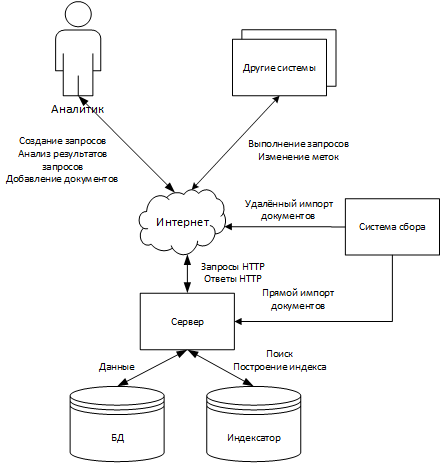
\includegraphics{design/domain}
\caption{Схема предметной области АИС.}
\label{figure:domain}
\end{figure}

\subsubsection{Сущности предметной области}

В процессе предварительного анализа предметной области были выделены следующие основные сущности:
\begin{itemize}
\item Документ;
\item Рубика;
\item Запрос;
\end{itemize}

А также дополнительные сущности, наличие которых следует из предыдущих:
\begin{itemize}
\item Метка документа;
\item Приложение документа;
\item Источник документа;
\item Операция системы -- долгосрочные операции над базой документов;
\item Настройки системы -- настройки пользователя.
\end{itemize}

\subsubsection{Перечень процессов, подлежащих автоматизации}
Автоматизации подлежат следующие процессы системы:
\begin{itemize}
\item Ввод документа в систему;
\item Построение ускоряющего поиск индекса;
\item Выполнение полнотекстового поиска на основе формализованного языка
запросов;
\item Просмотр документов и их редактирование;
\item Выполнение операций над индексом;
\item Рубрикация документов и сохранённых запросов;
\item Прогнозирование новостных потоков.
\end{itemize}

\subsubsection{Выбор и обоснование критериев качества}

Для данного программного изделия можно выделить следующие критерии качества:
\begin{itemize}
\item Удобство пользовательского интерфейса;
\item Качество полнотекстового поиска;
\item Дизайн рубрикатора;
\item Удобство интеграции с другими системами;
\item Возможность отмечать документы метками;
\item Качество прогноза.
\end{itemize}

\paragaph{Удобство пользовательского интерфейса.}
Означает простоту и понятность работы с системой. Оценивается:
\begin{itemize}
\item структура сайта (доступ к любой странице сайта требует не более трех кликов);
\item наличие сквозного меню (меню, которое присутствует на каждой странице сайта);
\item присутствие на всех страницах сайта ссылки на главную страницу;
\item иерархическая структурированность информации сайта, степень интуитивно понятного меню;
\end{itemize}

\paragraph{Качество полнотекстового поиска.}
Оценка релевантности найденной информации, скорость выполнения запроса, возможности формализованного языка запросов.

\paragraph{Дизайн рубрикатора.}
При оценке дизайна рубрикатора документов учитывается:
\begin{itemize}
\item Непосредственное наличие рубрикатора в стандартной поставке системы;
\item Стиль отображения древовидной структуры;
\item Отображение сохранённых запросов внутри рубрик;
\item Отображение информации о количестве документов в рубрике;
\end{itemize}

\paragraph{Удобство интеграции с другими системами.} 
Оценивается:
\begin{itemize}
\item Наличие интеграционного интерфейса;
\item Удобность этого интерфейса для разработчиков;
\item Полнота интерфейса (полная реализация всех возможностей системы в интерфейсе).
\end{itemize}

\paragraph{Возможность отмечать документы метками.}
Наличие возможности отмечать произвольными метками документы или сложность реализации такой возможности. Включает в себя:
\begin{itemize}
\item Поиск по наличию меток или по их отсутствию;
\item Удобство отображения для пользователя;
\item Возможность пользователю задавать метки документам;
\item Удобство интеграционного интерфейса для работы с метками.
\end{itemize}

\paragraph{Качество прогноза.}
При оценке качества прогноза новостного потока учитывается:
\begin{itemize}
\item Построение графиков количества документов, соответствующих сохранённому запросу, по дням;
\item Наличие ретроспективного прогноза;
\item Отображение аналитической функции прогноза;
\item Качество прогнозирования, возможность прогнозировать сложные потоки;
\end{itemize}

Присвоим критериям качества следующие весовые коэффициент, которые отображены в таблице~\ref{table:qualityWeights}.

\begin{table}[h!]
\centering
\caption{Критерии качества и их весовые коэффициенты}
\label{table:qualityWeights}
\begin{tabular}{L{10cm}|C{3cm}}
\multicolumn{1}{C{10cm}|}{Критерий} & 
\multicolumn{1}{C{3cm}}{$\alpha$} \\
\hline\hline

Удобство пользовательского интерфейса & 0.1 \\
Качество полнотекстового поиска & 0.4 \\
Дизайн рубрикатора & 0.1 \\
Удобство интеграции & 0.2 \\
Возможность отмечать документы метками & 0.1 \\
Качество прогноза & 0.1 \\

\end{tabular}
\end{table}

Выполнено следующее условие:
\begin{equation}
\sum \alpha_i = 0.1 + 0.4 + 0.1 + 0.2 + 0.1 + 0.1 = 1
\end{equation}

\subsubsection{Перечень задач, подлежащих решению в процессе разработки}

В процессе разработки необходимо решить следующие задачи:
\begin{itemize}
\item исследование и анализ предметной области;
\item анализ и определение критериев качества;
\item определение функциональных требований для разрабатываемой системы;
\item разработка структуры модулей системы, с выделением функциональности для каждого модуля;
\item проектирование базы данных: инфологической и даталогической модели;
\item оптимизация структуры базы данных;
\item рассмотрение и обоснование архитектурных особенностей реализации системы;
\item выбор программных библиотек для реализации модулей;
\item выбор и обоснование решения по организации отказоустойчивой модели хранения данных;
\item разработка интерфейса взаимодействия пользователя с программой;
\item реализация графа диалога;
\item написание и отладка программного кода модулей системы;
\item разработка технической документации.
\end{itemize}

\subsubsection{Анализ аналогов и прототипов}

Для расчета нормированного значения j-го варианта по i-ому критерию необходимо
воспользоваться формулой~\ref{equation:criteria}.

\begin{equation}
\label{equation:criteria}
K_{ij} = \frac{x_{ij} - x_i^-}{x_i^+ - x_i^-}
\end{equation}
\begin{ESKDexplanation}
\item[где ] $x_{ij}$ - натуральное значение;
\item       $x_i^+$ - максимальное значение;
\item       $x_i^-$ - минимальное значение.
\end{ESKDexplanation}

Для расчета интегрального показателя необходимо воспользоваться формулой~\ref{equation:criteriaTotal}.

\begin{equation}
\label{equation:criteriaTotal}
K = \sum_{i=1}^m \alpha_i K_{ij}
\end{equation}
\begin{ESKDexplanation}
\item[где ] $m$ - количество критериев.
\end{ESKDexplanation}

Оценка по критериям производится путём присуждения баллов в соответствии со шкалой, представленной в таблице~\ref{table:criteria}.

\begin{table}[h!]
\centering
\caption{Критерии качества и их весовые коэффициенты}
\label{table:criteria}
\begin{tabular}{L{4cm}|C{2cm}|C{2cm}|C{2cm}|C{2cm}|C{2cm}}
\multicolumn{1}{C{4cm}|}{Качественный показатель} & 
\multicolumn{1}{C{2cm}|}{Отлично} & 
\multicolumn{1}{C{2cm}|}{Хорошо} & 
\multicolumn{1}{C{2cm}|}{Удовлетворительно} & 
\multicolumn{1}{C{2cm}|}{Плохо} & 
\multicolumn{1}{C{2cm} }{Неудовлетворительно} \\
\hline\hline

Количественный показатель & 5 & 4 & 3 & 2 & 1 \\
$K_{ij}$ & 1 & 0.75 & 0.5 & 0.25 & 0 \\

\end{tabular}
\end{table}

Исследуем три системы аналогов:
\begin{itemize}
\item Elsatic search
\item Mircrosoft search server
\item ODB Text
\end{itemize}

Эти аналоги имеют ряд принципиальных недостатков и не могут отвечать всем
требованиям.

Недостатками аналога «Elsatic search» являются:
\begin{itemize}
\item отсутствие системы прогнозирования;
\item отсутствие готового интерфейса пользователя.
\end{itemize}

Недостатками аналога «Mircrosoft search server» являются:
\begin{itemize}
\item малое количество возможностей у формализованного языка запросов;
\item отсутствие сохранённых запросов в рубрикаторе;
\item отсутствие системы прогнозирования.
\end{itemize}

Недостатками аналога «ODB Text» являются:
\begin{itemize}
\item невозможность интеграции системы в комплекс;
\item слабая система прогнозирования;
\item отсутствие возможности отмечать документы метками;
\end{itemize}

Сравним аналоги и прототипы без учета весовых коэффициентов, результаты сведены в таблицу~\ref{table:analogs1}.

\begin{table}[h!]
\centering
\caption{Сравнение аналогов и прототипов без учета весовых коэффициентов}
\label{table:analogs1}
\begin{tabular}{L{4cm}|C{3cm}|C{3cm}|C{3cm}|C{3cm}}
\multicolumn{1}{C{4cm}|}{Критерий} & 
\multicolumn{1}{C{3cm}|}{Elastic Search} & 
\multicolumn{1}{C{3cm}|}{Microsoft SC} & 
\multicolumn{1}{C{3cm}|}{ODB Text} & 
\multicolumn{1}{C{3cm}}{Волхв} \\
\hline\hline

Удобство пользовательского интерфейса & 1 & 4 & 5 & 4 \\ \hline
Качество полнотекстового поиска & 5 & 3 & 3 & 5 \\ \hline
Дизайн рубрикатора & 1 & 3 & 4 & 5 \\ \hline
Удобство интеграции & 5 & 3 & 1 & 4 \\ \hline
Возможность отмечать документы метками & 4 & 5 & 1 & 5 \\ \hline
Качество прогноза & 1 & 1 & 3 & 5 \\ \hline
\hline
Итого & 17 & 19 & 17 & 28 \\

\end{tabular}
\end{table}

Сравним аналоги и прототипы с учетом весовых коэффициентов, результаты сведены в таблицу~\ref{table:analogs2}.

\begin{table}[h!]
\centering
\caption{Сравнение аналогов и прототипов без учета весовых коэффициентов}
\label{table:analogs2}
\begin{tabular}{L{3cm}|C{1cm}|C{3cm}|C{2cm}|C{3cm}|C{3cm}}
\multicolumn{1}{C{3cm}|}{Критерий} & 
\multicolumn{1}{C{1cm}|}{$\alpha$} & 
\multicolumn{1}{C{3cm}|}{Elastic Search} & 
\multicolumn{1}{C{2cm}|}{Microsoft SC} & 
\multicolumn{1}{C{3cm}|}{ODB Text} & 
\multicolumn{1}{C{3cm}}{Волхв} \\
\hline\hline

Удобство пользовательского интерфейса & 0.1 & 0 & 0.75 & 1 & 0.75 \\ \hline
Качество полнотекстового поиска & 0.4 & 1 & 0.5 & 0.5 & 1 \\ \hline
Дизайн рубрикатора & 0.1 & 0 & 0.5 & 0.75 & 1 \\ \hline
Удобство интеграции & 0.2 & 1 & 0.5 & 0 & 0.75 \\ \hline
Возможность отмечать документы метками & 0.1 & 0.75 & 1 & 0 & 1 \\ \hline
Качество прогноза & 0.1 & 0 & 0 & 0.5 & 1 \\ \hline
\hline
Итого & 1 & 0.675 & 0.525 & 0.425 & 0.925 \\

\end{tabular}
\end{table}

Таким образом, автоматизированная информационная система мониторинга и
прогнозирования новостных потоков «Волхв» является лучшим среди аналогов и
оправдывает свое создание.